\chapter{Design}\label{design}

\section{MoSCoW Statement}


    \subsection{Must have}
        \begin{itemize}
            \setlength\itemsep{1em}
            \item The application \textbf{must} be able to detect people in the given image or video.
            \item The application \textbf{must} be able to determind distancing between people in the given image or video.
            \item The application \textbf{must} save the processed image of video.
            \item The application \textbf{must} allow user to choose image or video from device's storage.
        \end{itemize}

    \subsection{Should have}
        \begin{itemize}
            \item The application \textbf{should} be able to stream video from camera.
            \item The application \textbf{should} be able to show detected people on camera.
            \item The application \textbf{should} support parallel computing.
        \end{itemize}

    \subsection{Could have}
        \begin{itemize}
            \item The application \textbf{could} choose computation options between sequencial or parallelism.
            \item The application \textbf{could} support NEON techonology.
            \item The application \textbf{could} be able to process the given tasks in background.
        \end{itemize}
    \subsection{Won't have}
        \begin{itemize}
            \item The application \textbf{won't} other objects which are not human.
            \item The application \textbf{won't} support GPU computation.
        \end{itemize}


\section{System Architecture}
    According to Figure~\ref{systemOverview}

    \begin{figure}[!ht]
        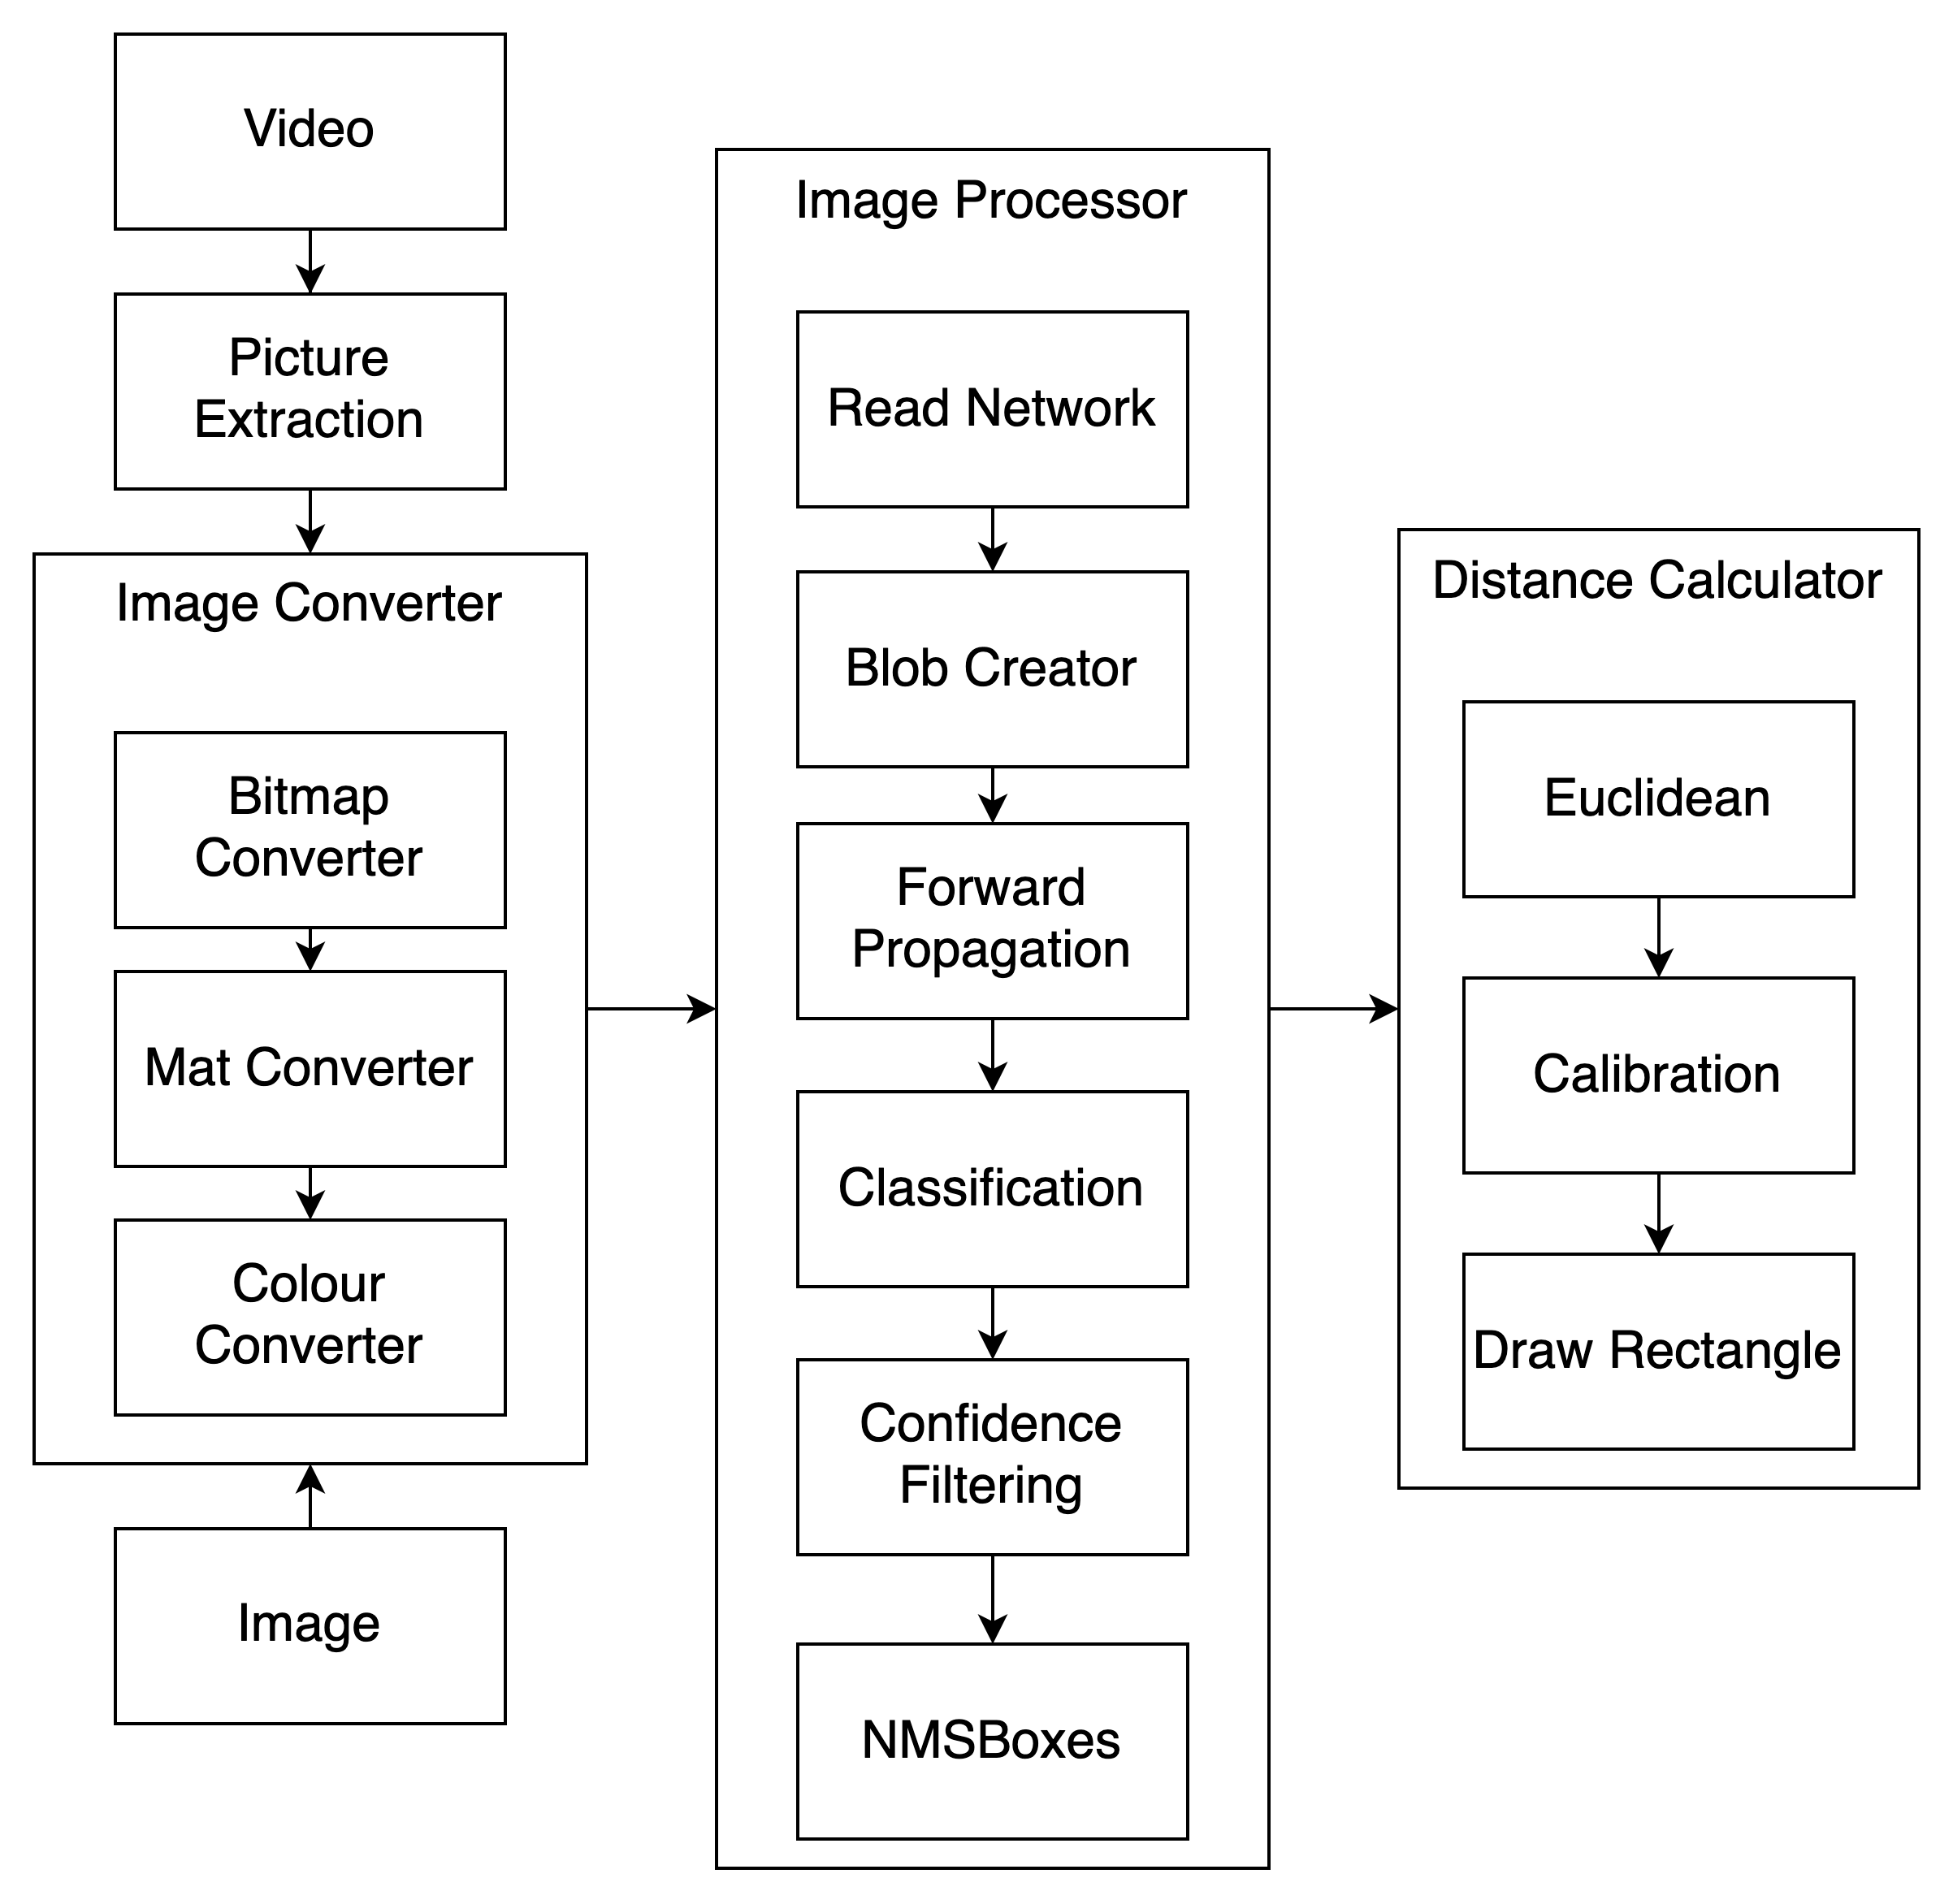
\includegraphics[width=6in]{images/chapter3/system-overview.png}
        \caption{System Overview Diagram}
        \label{systemOverview}
    \end{figure}

    \begin{figure}[!ht]
        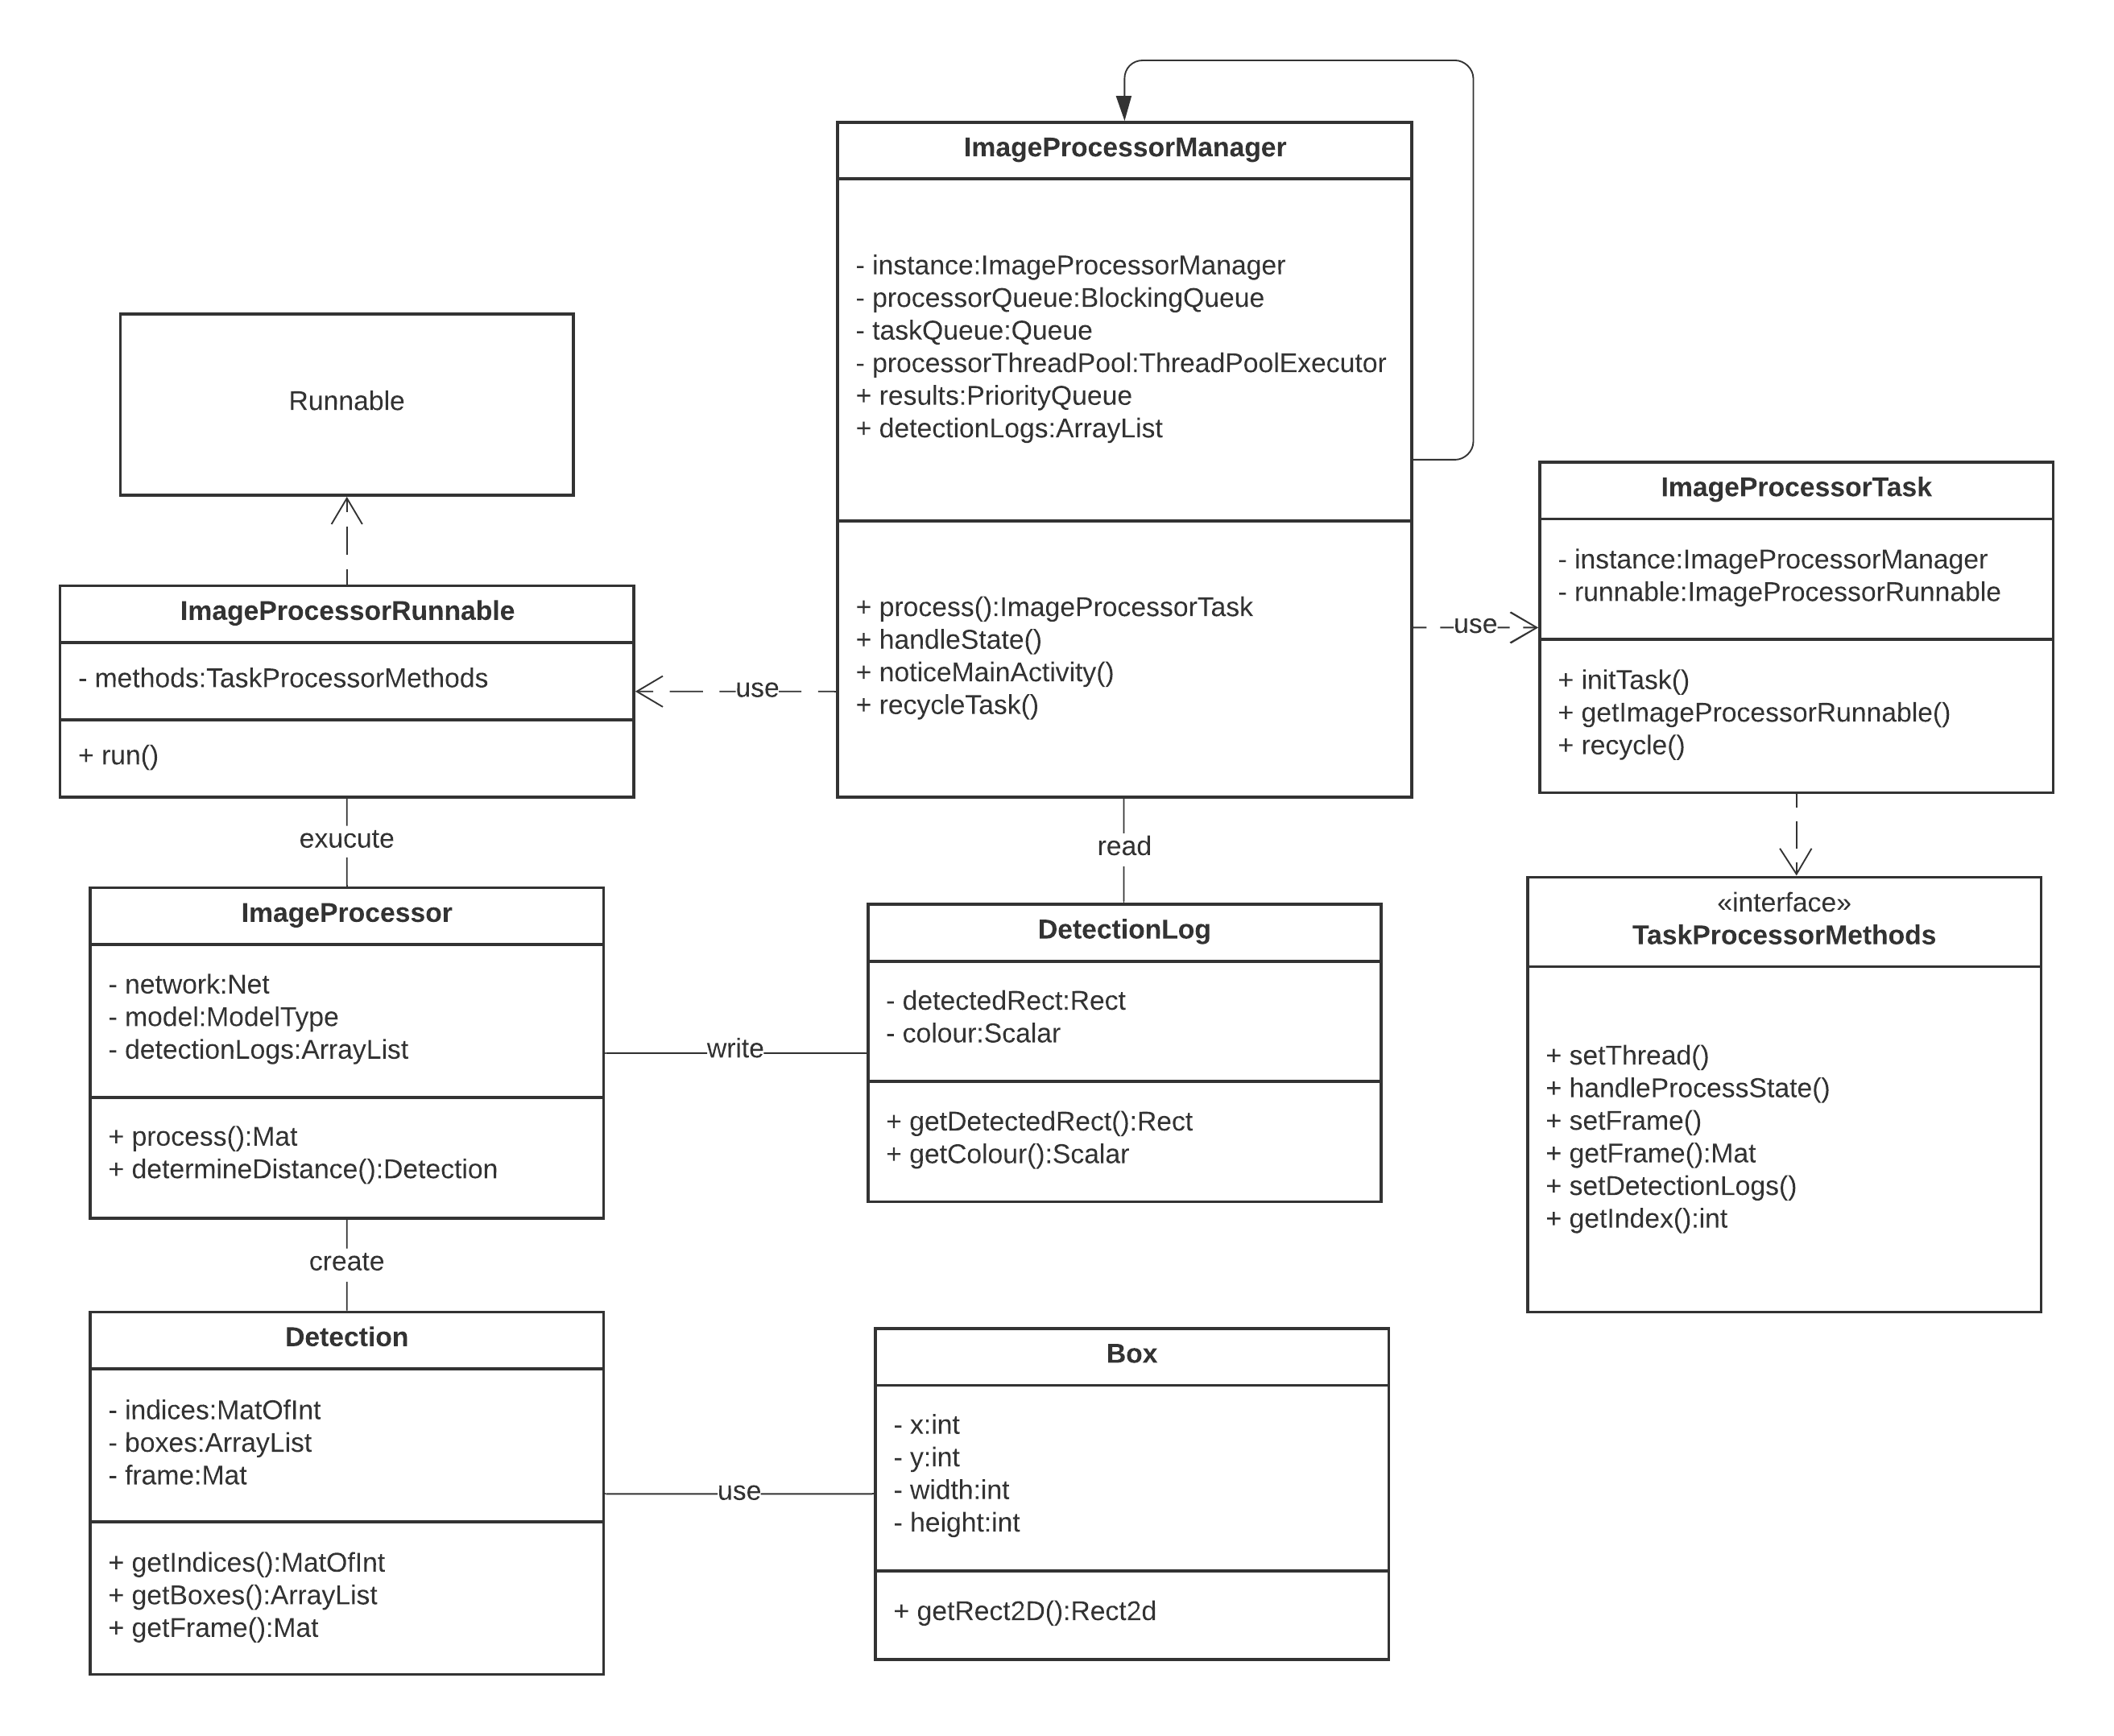
\includegraphics[width=6in]{images/chapter3/detection-uml.png}
        \caption{Detection UML Class}
        \label{detectionUml}
    \end{figure}

\section{Parallelism}
    \begin{figure}[!ht]
        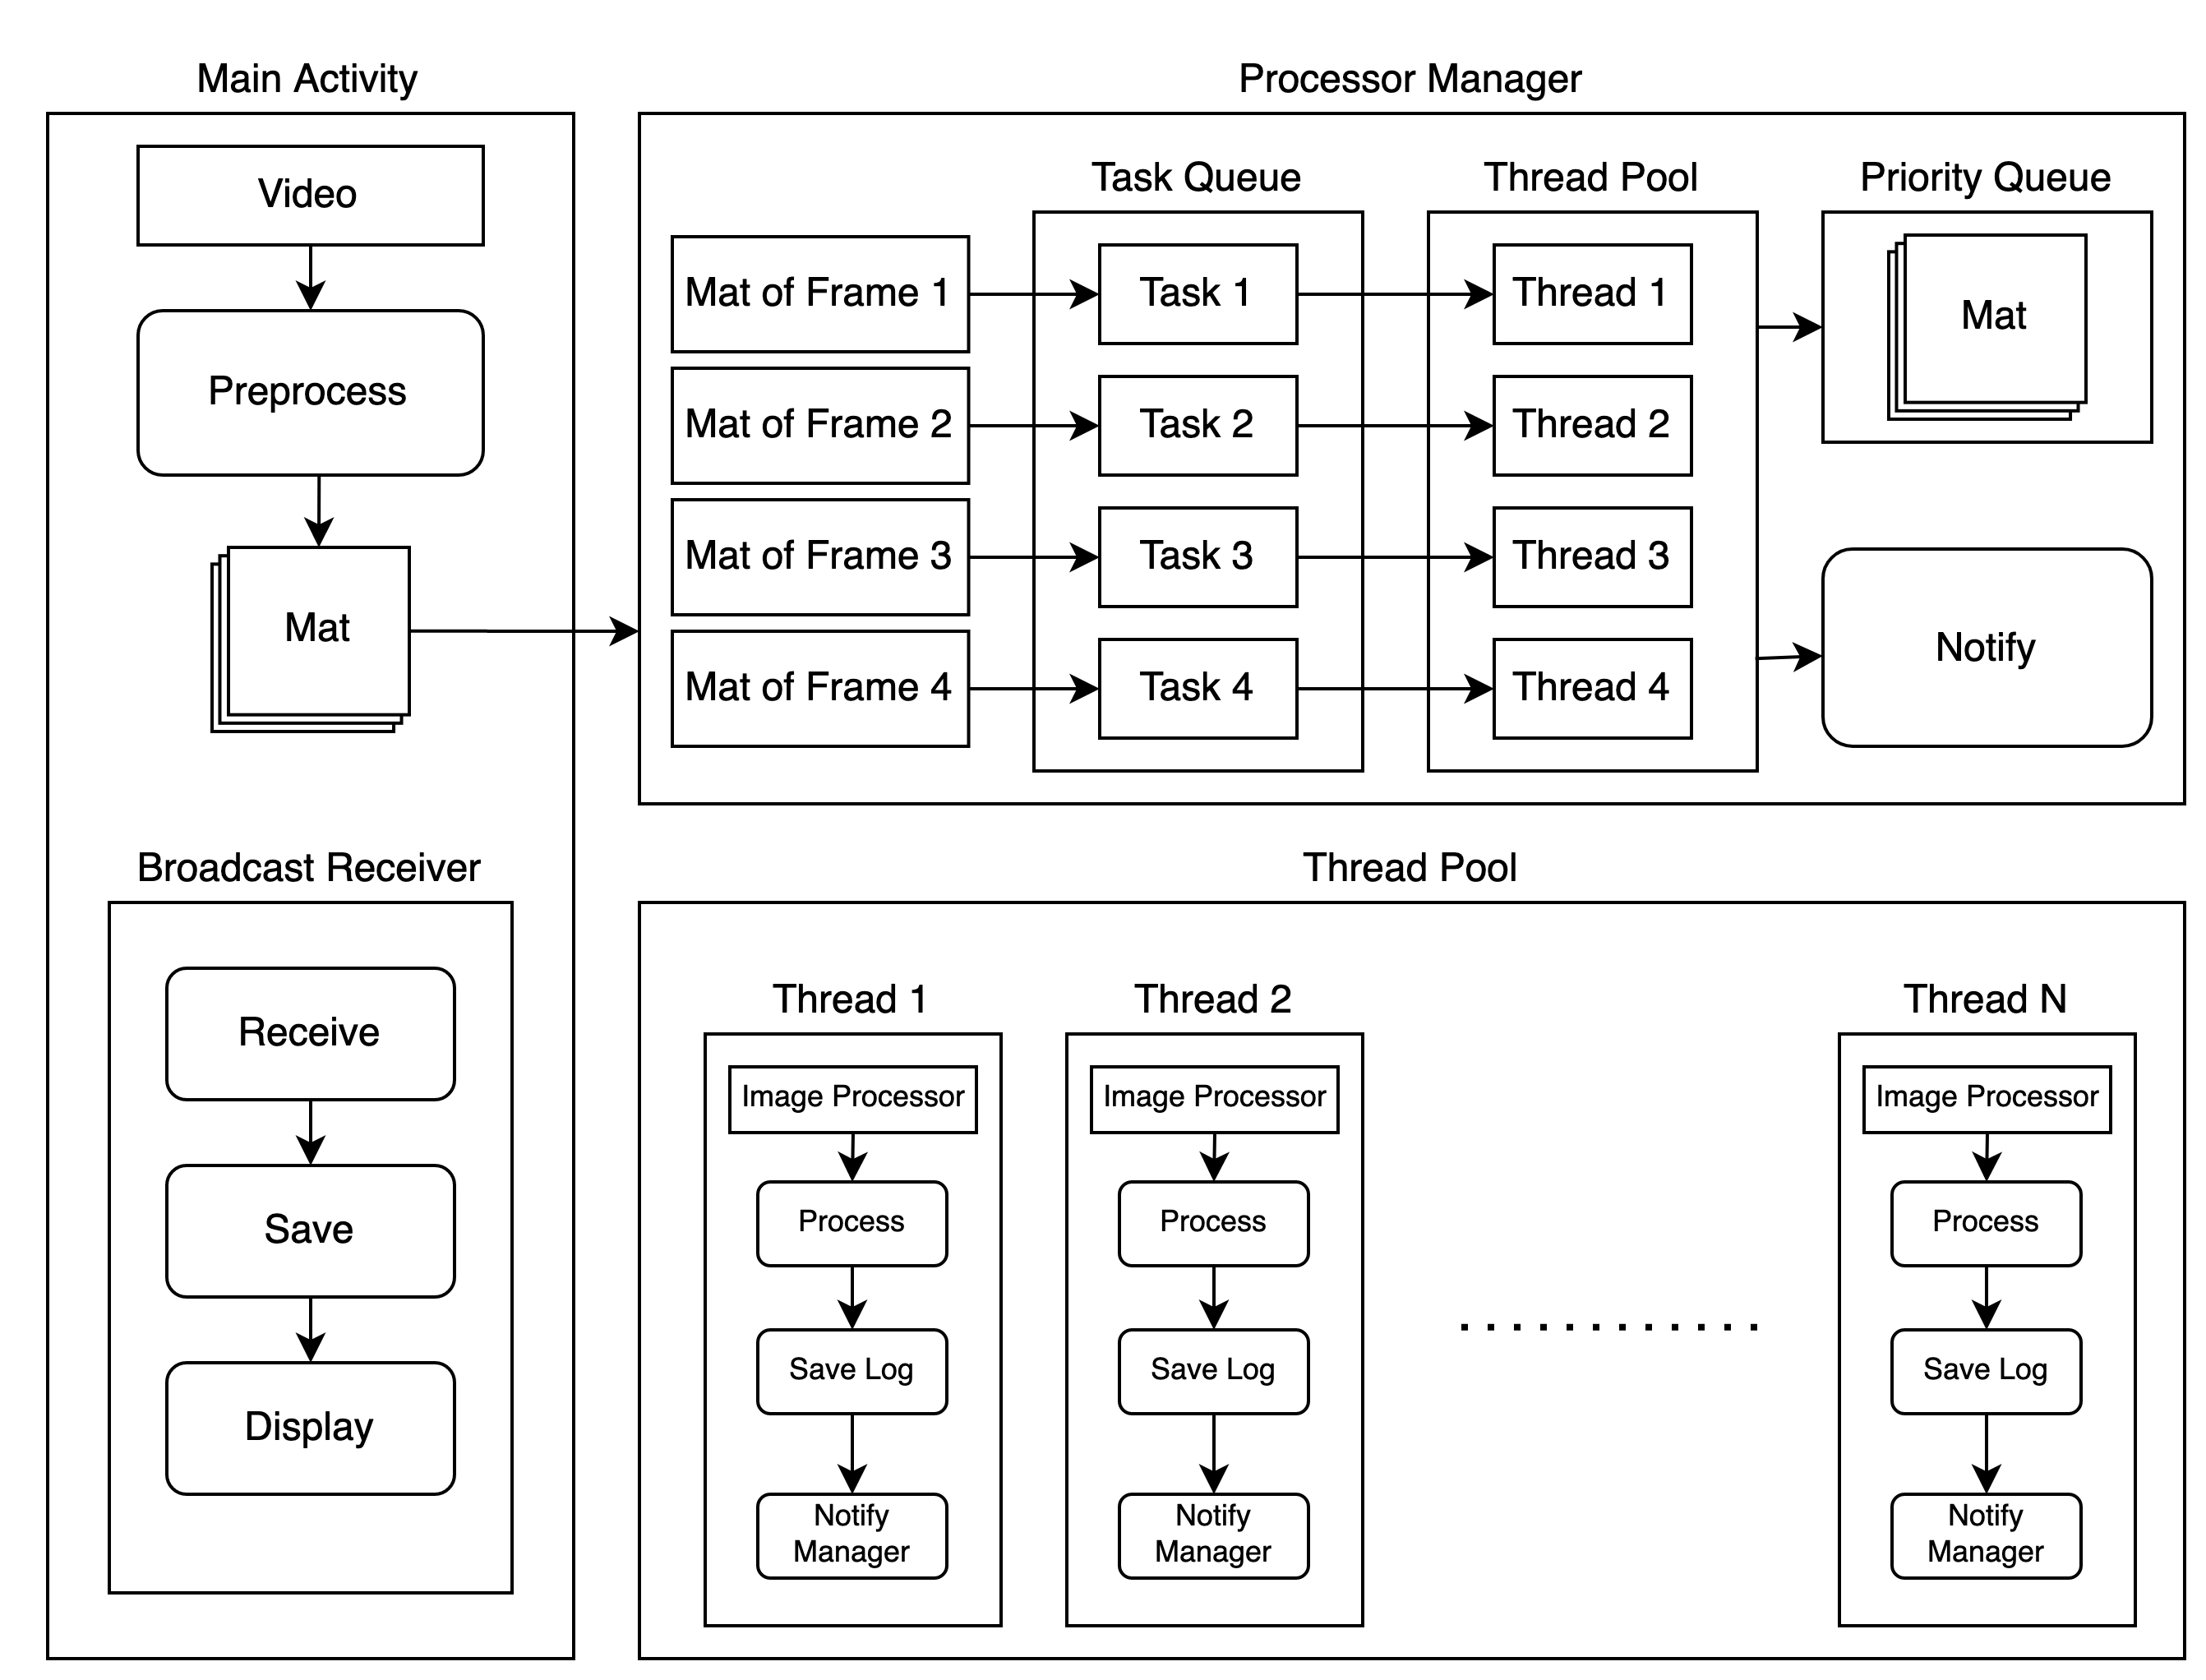
\includegraphics[width=6in]{images/chapter3/parallel.png}
        \caption{Parallel Computing Diagram}
        \label{systemOverview}
    \end{figure}
\section{Interface Design}